\resizebox{\textwidth}{!}{
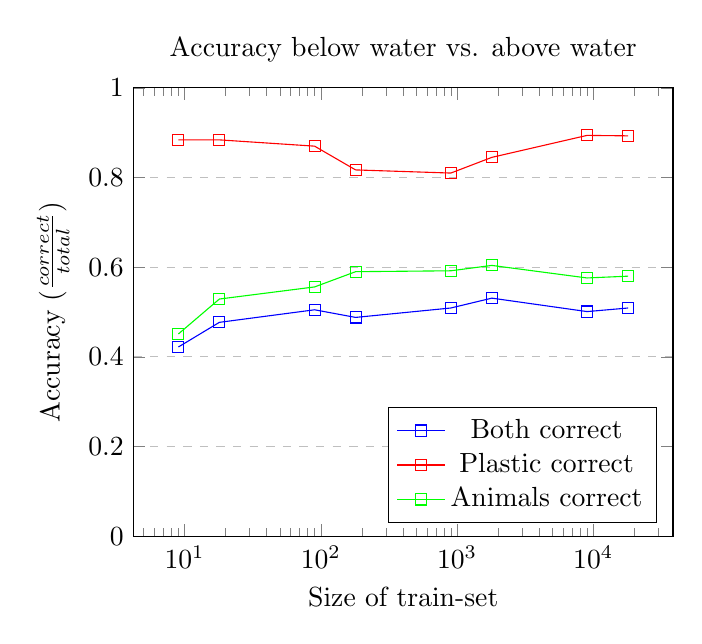
\begin{tikzpicture}
\begin{semilogxaxis}[
    title={Accuracy below water vs. above water},
    xlabel={Size of train-set},
    ylabel={Accuracy ($\frac{correct}{total}$)},
    %xmin=0, xmax=18000,
    ymin=0, ymax=1,
    legend pos=south east,
    ymajorgrids=true,
    grid style=dashed,
]
\addplot[
    color=blue,
    mark=square,
    ]
    coordinates {
    (9,0.422) (18,0.477) (90,0.505) (180,0.488) (900,0.509) (1800,0.531) (9000,0.501) (18000,0.509)
    };
    \addlegendentry{Both correct}
\addplot[
    color=red,
    mark=square,
    ]
    coordinates {
    (9,0.884) (18,0.884) (90,0.870) (180,0.817) (900,0.810) (1800,0.845) (9000,0.894) (18000,0.893)
    };
    \addlegendentry{Plastic correct}
\addplot[
    color=green,
    mark=square,
    ]
    coordinates {
    (9,0.451) (18,0.529) (90,0.556) (180,0.590) (900,0.592) (1800,0.604) (9000,0.576) (18000,0.580)
    };
    \addlegendentry{Animals correct}
\end{semilogxaxis}
\end{tikzpicture}
\hspace{.5cm}
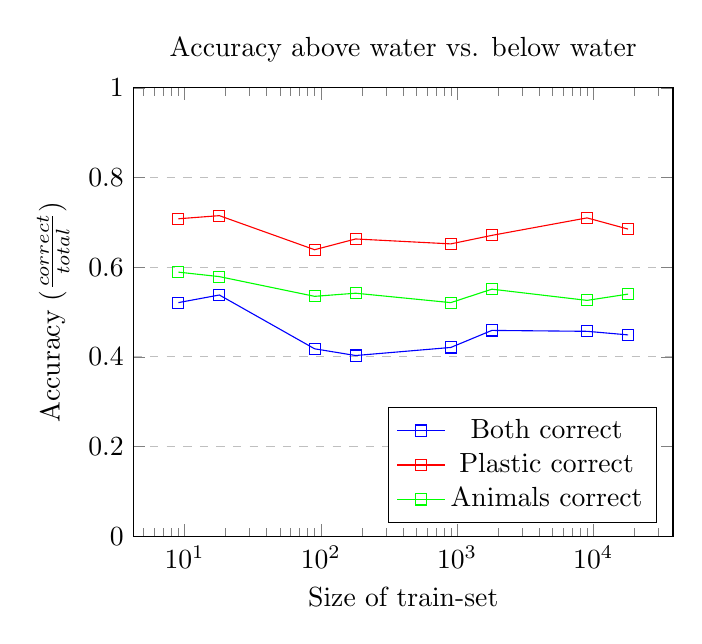
\begin{tikzpicture}
\begin{semilogxaxis}[
    title={Accuracy above water vs. below water},
    xlabel={Size of train-set},
    ylabel={Accuracy ($\frac{correct}{total}$)},
    %xmin=0, xmax=18000,
    ymin=0, ymax=1,
    legend pos=south east,
    ymajorgrids=true,
    grid style=dashed,
]
\addplot[
    color=blue,
    mark=square,
    ]
    coordinates {
    (9,0.521) (18,0.538) (90,0.418) (180,0.403) (900,0.421) (1800,0.459) (9000,0.457) (18000,0.449)
    };
    \addlegendentry{Both correct}
\addplot[
    color=red,
    mark=square,
    ]
    coordinates {
    (9,0.708) (18,0.715) (90,0.639) (180,0.663) (900,0.652) (1800,0.671) (9000,0.710) (18000,0.685)
    };
    \addlegendentry{Plastic correct}
\addplot[
    color=green,
    mark=square,
    ]
    coordinates {
    (9,0.589) (18,0.579) (90,0.535) (180,0.542) (900,0.521) (1800,0.551) (9000,0.526) (18000,0.540)
    };
    \addlegendentry{Animals correct}
\end{semilogxaxis}
\end{tikzpicture}
}